\chapter{Princip fungování Pletačka IoT}
V~předchozích kapitolách byly popsány jednotlivé část systému Pletačka IoT.
V~této kapitole bude celý systém popsán jako celek.


\section{Sběr dat}
První, a~tou nejdůležitější částí, je získávání dat pomocí senzorů.
Jakmile senzor zaznamená jakoukoliv změnu, okamžitě tuto zprávu odesílá na server.
Odesílání probíhá skrze senzorové API, kde se nejdříve senzor ověří a~následně se stav zapíše do databáze k~příslušnému senzoru.
Po zapsání do databáze se vrátí do senzoru zpráva o~provedení zápisu. 


\section{Vyhodnocování dat}
Dalším krokem je zpracovávání surových dat z~databáze.
K~tomuto účelu běží na serveru výběrové API, které je automaticky spouštěné v~nastavený čas.
Jde o~generování širších výběrů dat, hodinové, denní, měsíční a~roční výběry.
Tyto výběry se následně ukládají do databáze k~danému senzoru.
Generování těchto dat probíhá převážně v~noci, kdy je server nejméně vytížen.


\section{Zobrazování dat}
Posledním krokem je zobrazení dat uživateli.
Je to jediná část, se kterou se běžný uživatel dostane do kontaktu.
Proto je nutné, aby zobrazení bylo co nejrychlejší a~pro uživatele co nejpříjemnější.
% K~rychlému zobrazování se využívají předgenerované výběry, ke kterým se rychle dopočítají nově nasbíraná data.
K~rychlému zobrazování se využívají předgenerované výběry, ke kterým se dopočítají dosud nezpracovaná data a~celý výsledek se zobrazí uživateli.


% \fxnote[author=JPA]{\textcolor{mygreen}{"se rychle dopočítají nově nasbíraná data" - jaká data se dopočítávají => vice rozepsat}}


% \fxnote[author=JA]{\textcolor{mygreen}{schéma sběr - vyhodnocení - zobrazení}}

\begin{figure}[htbp]
    \centering
    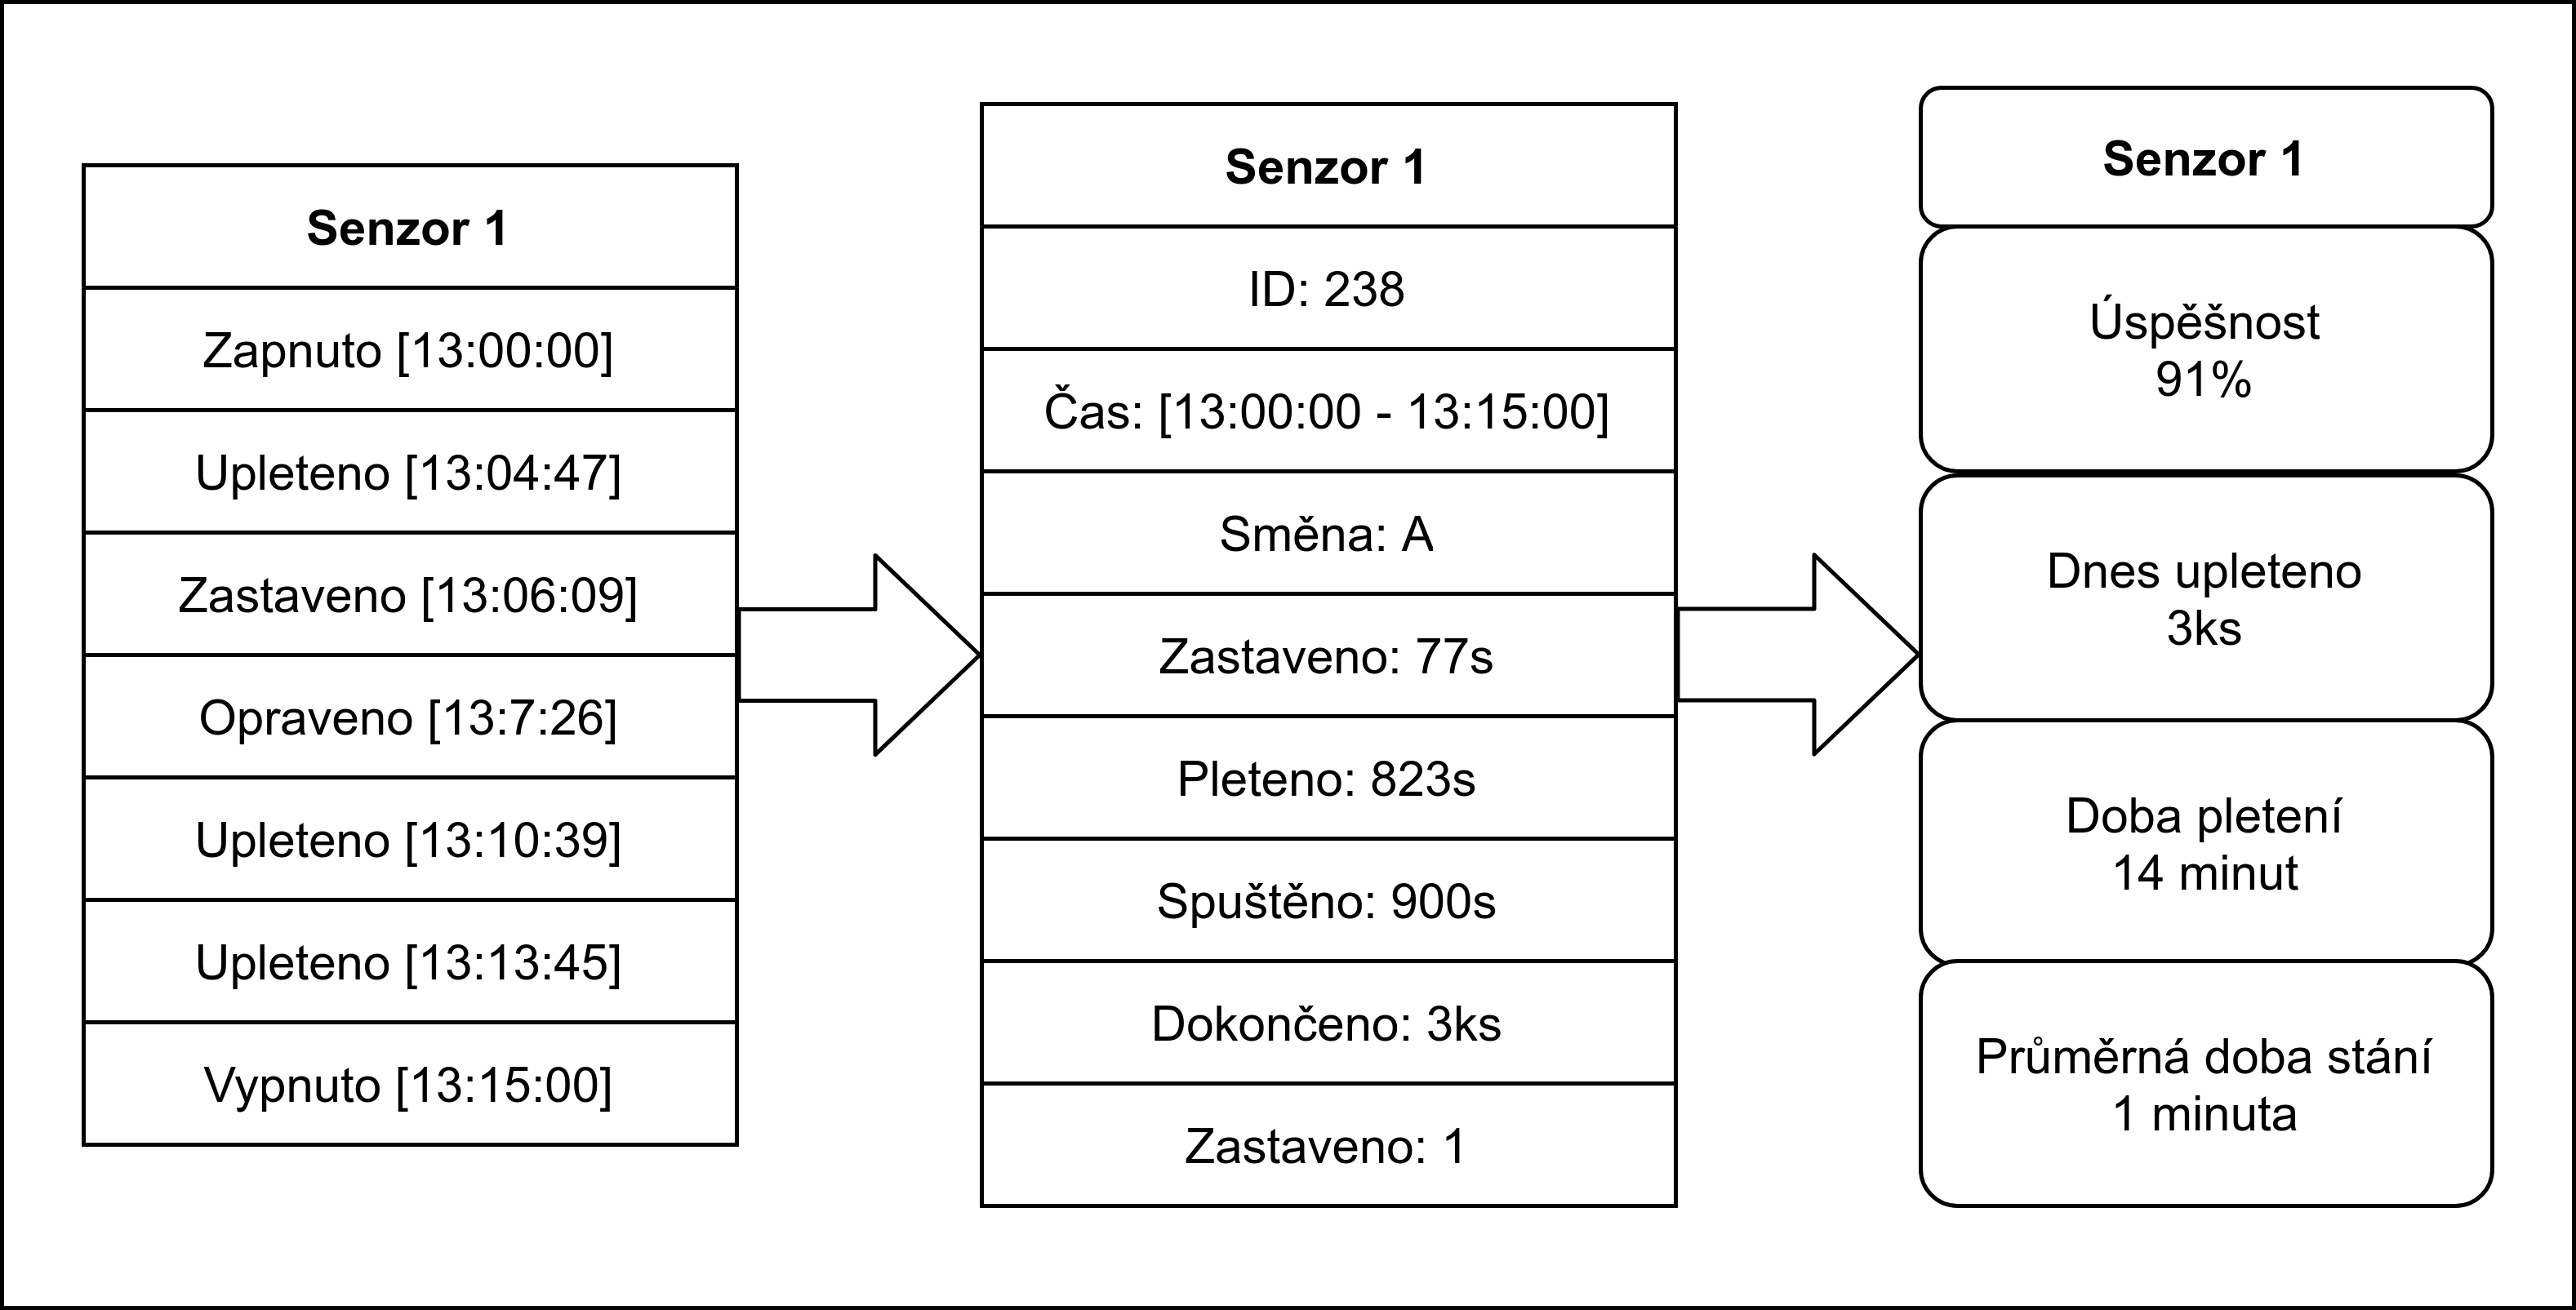
\includegraphics[width=\textwidth]{img/Princip.png}
    \caption{Zpracování dat}
    \label{fig:princip}
\end{figure}

\section{Konektivita}
Webové stránky se dají jednoduše zobrazit na počítači~či~notebooku.
Stránky jsou responzivní a~lze je používat i~na mobilních zařízeních.
Přístup k~webu je pouze z~vnitřní sítě firmy, to zajišťuje základní bezpečnost pro systém.


\newpage